\scanpage{20}\mspage{19}
of this type if $L$ is finite). Thus we shall therefore restrict ourselves to those $\unsure{\mathscr{L}|\Phi}\in\unsure{\mathcal F|\mathscr F}$ such that the $A\in\mathscr{L}$ are closed subsets of $L$, i.e. such that
\[ \mathscr{L}\subset\unsure{\mathcal P|\mathfrak P}_{\text{closed}}(L) \]
The \unsure{element|elements} of $\mathcal F'$ thus \unsure{obtained|obtained} can be interpreted in terms of $X$, as admissible families \inserted{(yes indeed)} of families of
\inserted{closed} subsets of $X$, \inserted{each} \uline{stable} under the equivalence relation of the open \deleted{cells} \inserted{strata} $X_{\unsure{\circ|a|\bullet|\cdot}}^\circ$, i.e. each a union of closed strata of $X$.
In a terminology which will be developed, they therefore all \deleted{are}\inserted{admit} the given covering of $X$ as a ``subdivision''\unsure{;|,} (or \unsure{earlier|rather}, \inserted{the one} induced on their support in $X$)

\figure{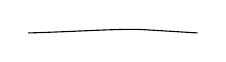
\begin{tikzpicture}\draw (0,0) .. controls (0.7,0.02) and (1.2,0.06) .. (1.5,0.04) -- (2.15,0);\end{tikzpicture}}

Let $\deleted{\unsure{\Phi}}F$ and $G$ be two set-theoretic figures of $L$. We want to define when $F$ is a \uline{refinement}, and when it is a \uline{subdivision} of $G$.

\uline{Proposition} Equivalent conditions

% slanted
\margin{This implies $|\deleted{\unsure{A}}F|\subset|G|$}
a) $[$ $\forall\unsure{a|\cdot}\;A\in F$, denoting by $G\deleted{{}_A}{}^A$ the set of $B\in G$ such that $A\subset B$, $G\deleted{{}_A}{}^A$ has a least
element $\varphi(A)$. (We thus find a map $\varphi:\deleted{\unsure{A}}F\longrightarrow G$, which is of course increasing.) $]$ Moreover
